% Copyright: Riley Taylor, Ethan Barnes, Deniz Misirlioglu, Jared Rozell
% ECE 345 final LaTex document
% 12/1/22
% Packages provided by open-source code.
\documentclass{article}
\usepackage[left=3cm,right=3cm,top=0cm,bottom=2cm]{geometry} % page settings
\usepackage{amsmath} % provides many mathematical environments & tools
\usepackage[framed,numbered,autolinebreaks,useliterate]{mcode}
\usepackage{graphicx}
\usepackage{relsize}
\usepackage{mathtools}
\usepackage{mcode}
\usepackage{booktabs}
\setlength{\parindent}{0mm}
%%%%%%%%%%%%%%%%%%%%%%%%%%%%%%%%%%%%%%%%%%%%%%%%%%%%%%%%%
%%%%%%%%%%%%%%%%%%% Title Page %%%%%%%%%%%%%%%%%%%%%%%%%%
%%%%%%%%%%%%%%%%%%%%%%%%%%%%%%%%%%%%%%%%%%%%%%%%%%%%%%%%%

% Miami graphic
\begin{document}
\begin{figure}
\vspace*{3cm}
  \hfill
\includegraphics[width=4in]{MiamiMcropped.png}\hspace*{\fill}
\end{figure}
\title{%
  \vspace*{.3cm}
  \huge
  Central Limit Theorem and Different Estimators \\
  \vspace*{1cm}
  \large College of Engineering and Computing \\
  \vspace*{.3cm}
	ECE 345: Engineering Statistics Final Project \\
 \vspace*{.3cm}
	Professor: Dr. Zhou \\
 \vspace*{.3cm}
	December 1, 2022
\vspace*{.3cm}}

\author{
Ethan Barnes
\texttt{barnese6@miamioh.edu}
\and
Deniz Misirlioglu
\texttt{misirld@miamioh.edu}
\and
Jared Rozell
\texttt{rozellj@miamioh.edu}
\and
Riley Taylor
\texttt{taylo550@miamioh.edu}
}
\date{}
\maketitle
\newpage
\vspace*{1cm}
%%%%%%%%%%%%%%%%%%%%%%%%%%%%%%%%%%%%%%%%%%%%%%%%%%%%%%%%%
%%%%%%%%%%%%%%%%%%%%%% Part A %%%%%%%%%%%%%%%%%%%%%%%%%%%
%%%%%%%%%%%%%%%%%%%%%%%%%%%%%%%%%%%%%%%%%%%%%%%%%%%%%%%%%
\section*{A) Approximate Theoretical PDF Using Arithmetic Mean}
First we solved for the random variable X in the equation $Y = X^2$. This allows us to find the pdf of x with respect to y. Solving the equation gives us:
\[
\mathlarger{Y = X^2}
\]
\[
\mathlarger{X = \pm\sqrt{Y}}
\]
Then we solved for the expectation of Y:
\[
\mathlarger{\mathlarger{E(A_n) = E(Y) = \int_{0}^{\infty} yf_Y (y)dy}}
\]
\[
\mathlarger{\mathlarger{E(Y) = \int_{0}^{\infty}y\frac{1}{\sigma\sqrt{2\pi y}}e^{-\frac{1}{2}(\frac{y}{\sigma^2})}dy = \sigma_x^2}}
\]
\[
\mathlarger{\mathlarger{V(Y) = \int_{0}^{\infty}(y-\sigma^2)^2\frac{1}{\sigma\sqrt{2\pi y}}e^{-\frac{1}{2}(\frac{y}{\sigma^2})}dy = 2\sigma_x^4}}
\]
\\
The pdf of x with respect to y will result in the following:
\[
\mathlarger{\mathlarger{f_x(y) = \frac{1}{\sqrt{2\pi}\sigma}e^{-\frac{1}{2}(\frac{x-\mu}{\sigma})^2}, \mu = 0}}
\]
\[
\mathlarger{\mathlarger{f_x(y) = \frac{1}{\sqrt{2\pi}\sigma}e^{-\frac{x^2}{2\sigma^2}}, x^2 = y}}
\]\\\\
The complete derived equation:
\[
\mathlarger{\mathlarger{f_x(y) = \frac{1}{\sqrt{2\pi}\sigma}e^{-\frac{y}{2\sigma^2}}, y > 0}}
\]
\\\\
According to the central limit theorem the approximate theoretical pdf of An is shown as follows:
\[
\mathlarger{\mathlarger{f(A_n) = \frac{1}{\sqrt{2\pi}\sigma_{A_n}}e^{-\frac{(A_n-\mu_{A_n})^2}{2\sigma_{A_n}^2}}, x^2 = y}}
\]
Using the following values of n = 2, 3, 16, 144:
\[
\mathlarger{\mathlarger{f(A_2)=N(\sigma_X^2,\sigma_X^4),y > 0}}
\]
\[
\mathlarger{\mathlarger{f(A_3)=N(\sigma_X^2,\frac{2\sigma_X^4}{3}),y > 0}}
\]
\[
\mathlarger{\mathlarger{f(A_{16})=N(\sigma_X^2,\frac{\sigma_X^4}{8}),y > 0}}
\]
\[
\mathlarger{\mathlarger{f(A_{144})=N(\sigma_X^2,\frac{\sigma_X^4}{72}),y > 0}}
\]

\newpage
\vspace*{1cm}
%%%%%%%%%%%%%%%%%%%%%%%%%%%%%%%%%%%%%%%%%%%%%%%%%%%%%%%%%
%%%%%%%%%%%%%%%%%%%%%% Part B %%%%%%%%%%%%%%%%%%%%%%%%%%%
%%%%%%%%%%%%%%%%%%%%%%%%%%%%%%%%%%%%%%%%%%%%%%%%%%%%%%%%%
\section*{B) True PDF of $A_n$ for $n=2$ Without Approximation}
\[
\mathlarger{\mathlarger{f({A_n}) = \frac{1}{\sqrt{2\pi}\sigma^2}e^{-\frac{((\frac{1}{2}(y_1+y_2))-\sigma^2)^2}{2\sigma^4}}, y>0}}
\]
\\
Calculating the bounds so we can solve for the pdf:
\[
\mathlarger{y > 0}
\]
\[
\mathlarger{z - y > 0}
\]
\center $y<z$ and $y>0$, resulting in $0 > y > z$
\center $A_2 = \frac{1}{2}(y_1+y_2)$, transforming into $Z = X + Y$
\\
\[
\mathlarger{\mathlarger{f_z(z)=\int\int_{x+y=z}f_{xy}(x,y)dxdy}}
\]
\\
\raggedright Since x and y are independent:
\[
\mathlarger{\mathlarger{f_z(z)=\int\int_{x+y=z}f_x(x)f_y(y)dxdy}}
\]
\\
\raggedright Resulting in a convolution integral of:
\[
\mathlarger{\mathlarger{f_z(z)=\int f_y(y)f_y(z-y)dy}}
\]
\\
\raggedright Implementing the bounds:
\vspace{0.35cm}
\[
\mathlarger{\mathlarger{\int_{0}^{z}f_y(y)f_y(z-y)dy}}
\]
\vspace{0.5cm}
\[
\mathlarger{\mathlarger{f_y(y)= \frac{1}{\sqrt{2\pi y}\sigma}e^{-\frac{y}{2\sigma^2}}, y>0}}
\vspace{1cm}
\]
\[
\mathlarger{\mathlarger{f(A_2)=f(z)=\int_{0}^{z}\frac{1}{\sqrt{2\pi y}\sigma}e^{-\frac{y}{2\sigma^2}}\frac{1}{\sqrt{2\pi (z-y)}\sigma}e^{-\frac{(z-y)}{2\sigma^2}}dy}}
\]
\vspace{0.5cm}
\[
\mathlarger{\mathlarger{=\int_{0}^{z}\frac{1}{\sqrt{2\pi y}\sigma}\frac{1}{\sqrt{2\pi (z-y)}\sigma}e^{-\frac{z}{2\sigma^2}}dy}}
\]
\vspace{0.5cm}
\[
\mathlarger{\mathlarger{=e^{-\frac{z}{2\sigma^2}}\int_{0}^{z}\frac{1}{\sqrt{2\pi y}\sigma}\frac{1}{\sqrt{2\pi (z-y)}\sigma}dy}}
\]
\vspace{0.5cm}
\[
\mathlarger{\mathlarger{\boxed{=\frac{e^{-\frac{z}{2\sigma^2}}}{2\sigma^2}}}}
\]

\newpage
\vspace*{1cm}
%%%%%%%%%%%%%%%%%%%%%%%%%%%%%%%%%%%%%%%%%%%%%%%%%%%%%%%%%
%%%%%%%%%%%%%%%%%%%%%% Part C %%%%%%%%%%%%%%%%%%%%%%%%%%%
%%%%%%%%%%%%%%%%%%%%%%%%%%%%%%%%%%%%%%%%%%%%%%%%%%%%%%%%%
\section*{C) Matlab Simulation for the PDF 
of $A_n$}
%%% Figure 2, C part 1 %%%
Standard Deviation (n=2) = 0.9328
\begin{figure}[h!]
\centering
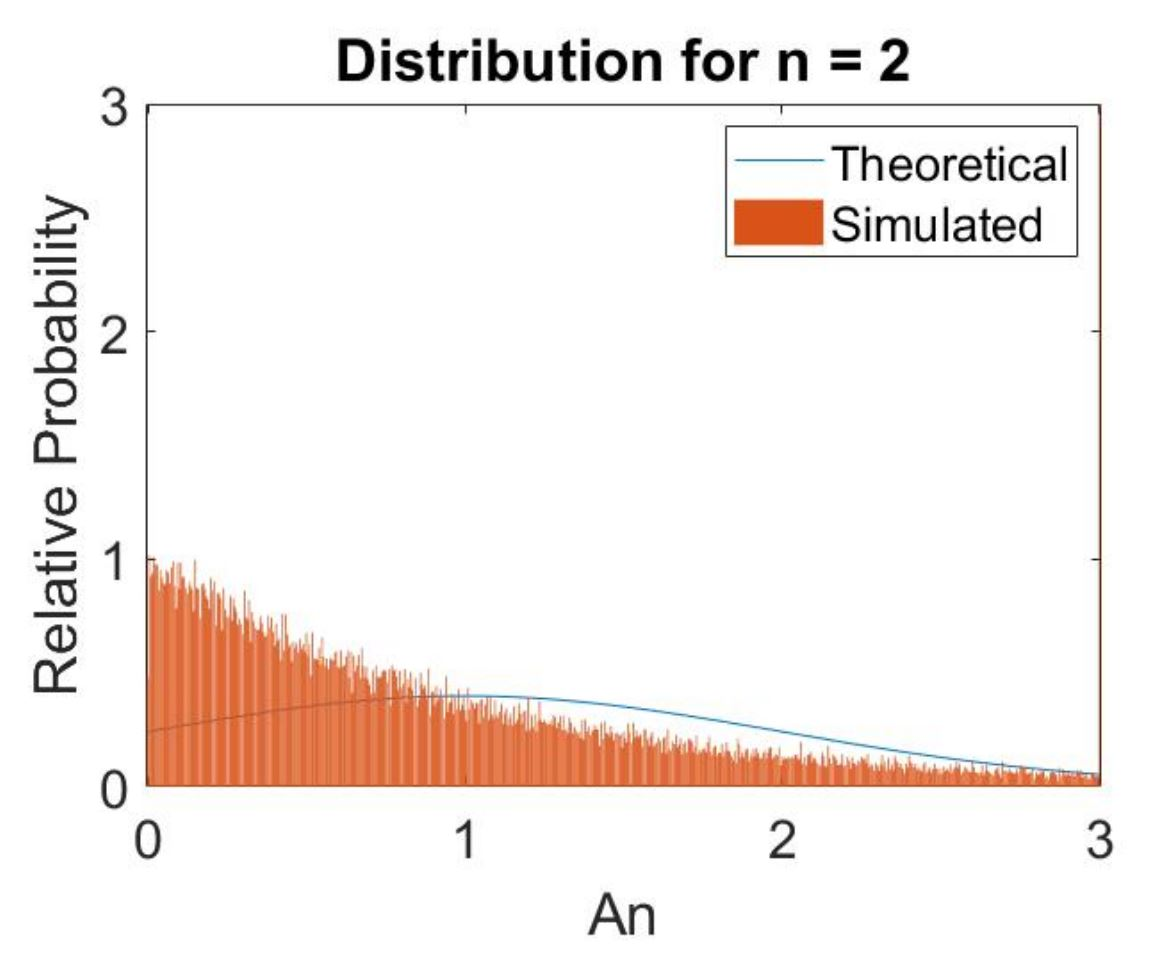
\includegraphics[scale=0.75]{Cpart1.jpg}
\caption{Simulated and Theoretical graph for $n = 2$}
\end{figure}

%%% Figure 3, C part 1_2 %%%
Standard Deviation (n=3) = 0.7645
\begin{figure}[h!]
\centering
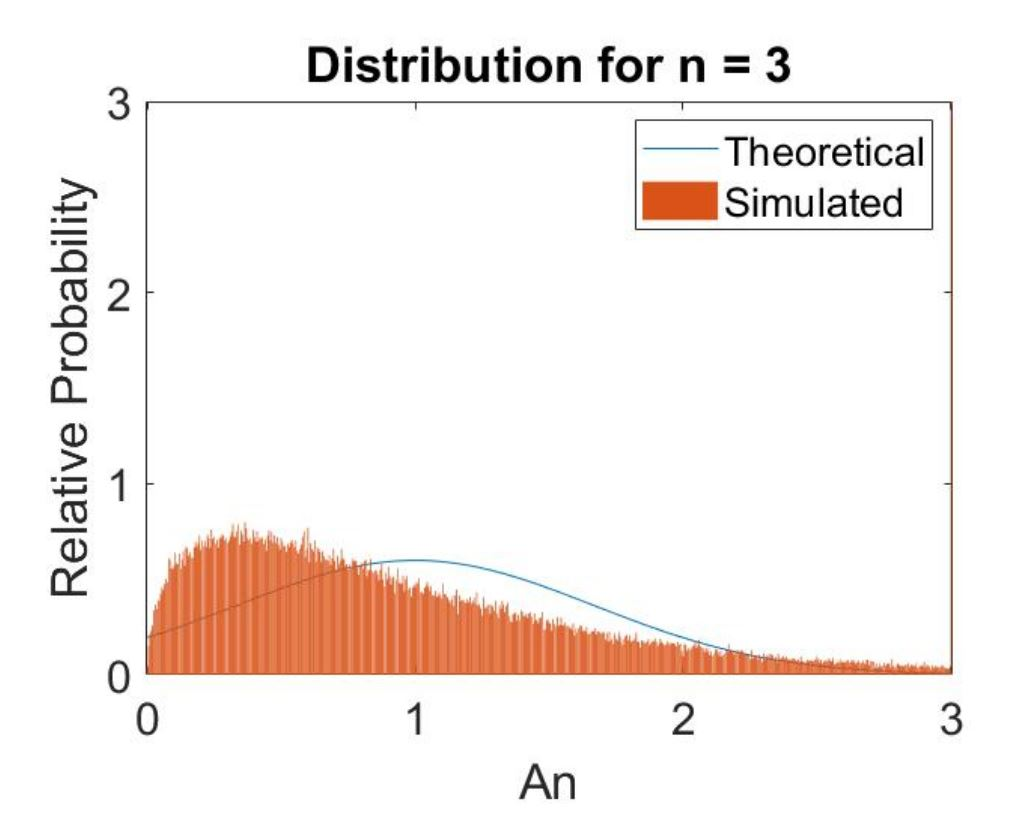
\includegraphics[scale=0.9]{Cpart1_2.jpg}
\caption{Simulated and Theoretical graph for $n = 3$}
\end{figure}

%%% Figure 4, C part 1_3 %%%
\vspace*{1.5cm}
Standard Deviation (n=16) = 0.3295
\begin{figure}[h!]
\centering
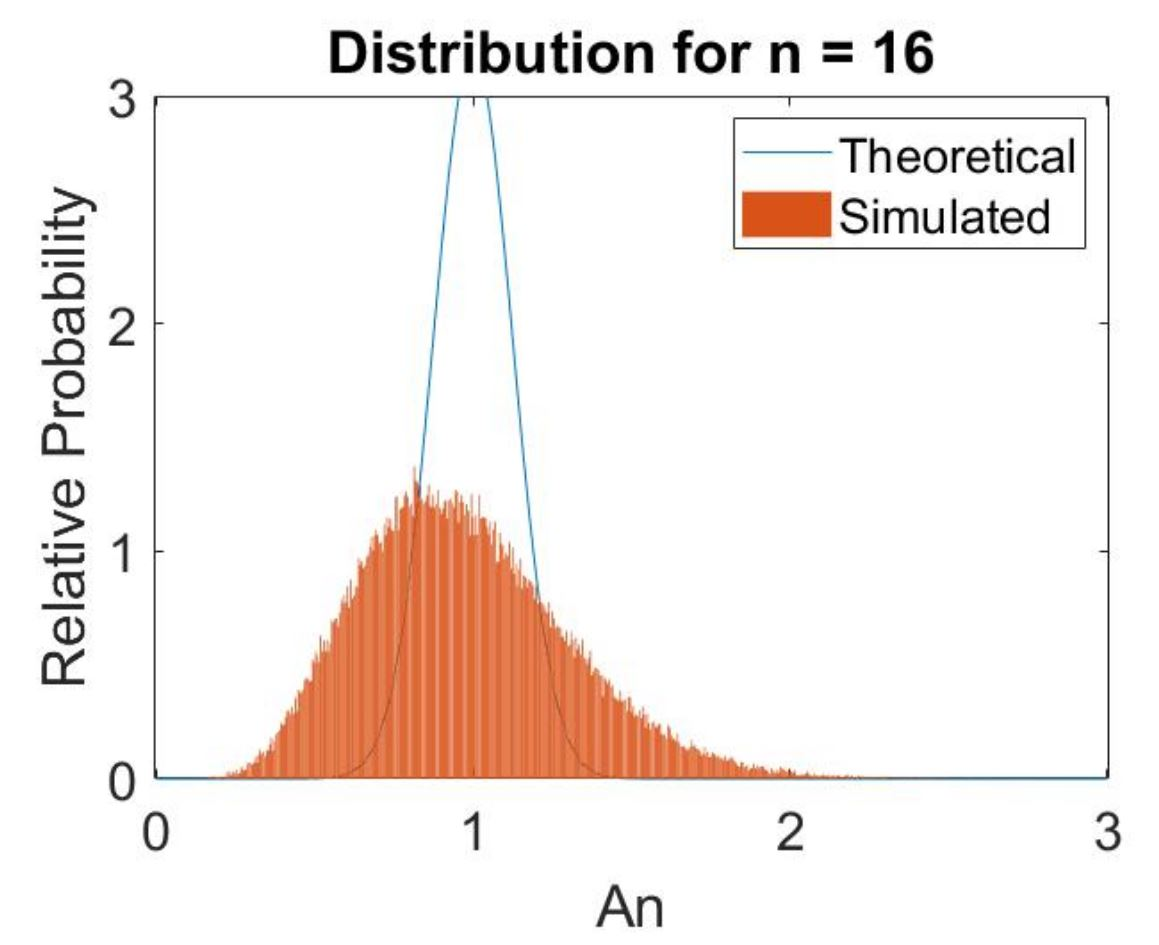
\includegraphics[scale=0.8]{Cpart1_3.jpg}
\caption{Simulated and Theoretical graph for $n = 16$}
\end{figure}

%%% Figure 5, C part 1_4 %%%
Standard Deviation (n=144) = 0.1100
\begin{figure}[h!]
\centering
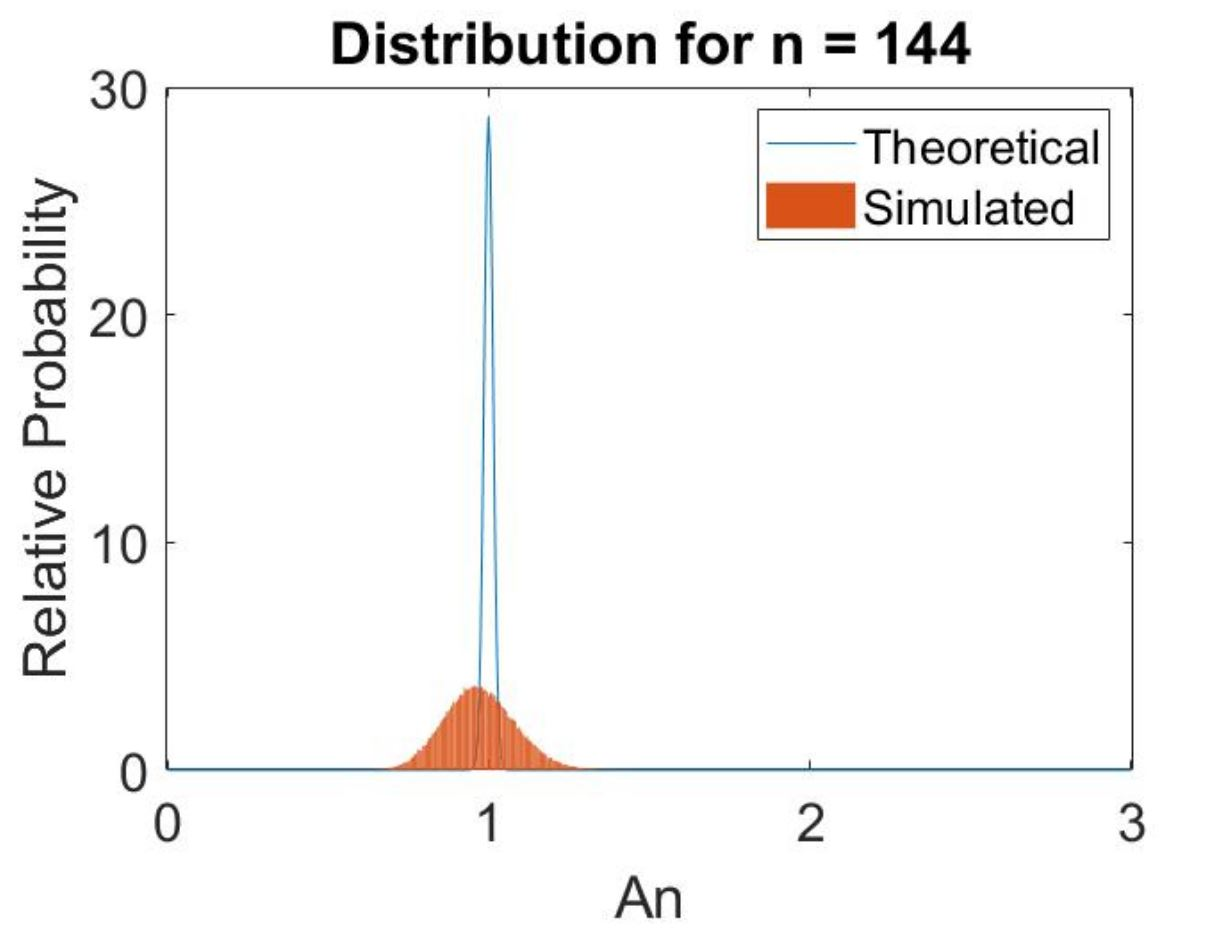
\includegraphics[scale=0.8]{Cpart1_4.jpg}
\caption{Simulated and Theoretical graph for $n = 144$}
\end{figure}

\newpage
\vspace*{1cm}
%%%%%%%%%%%%%%%%%%%%%%%%%%%%%%%%%%%%%%%%%%%%%%%%%%%%%%%%%
%%%%%%%%%%%%%%%%%%%%%% Part D %%%%%%%%%%%%%%%%%%%%%%%%%%%
%%%%%%%%%%%%%%%%%%%%%%%%%%%%%%%%%%%%%%%%%%%%%%%%%%%%%%%%%
\section*{D) Comparing the Three PDFs}
The theoretical distribution is normal and its mean is slightly larger than 1. The other two distributions appear to be a decaying exponential. The simulated distribution follows the shape of the true PDF, but is more biased towards 0. CLT is used to find the theoretical PDF, this approximation is most likely the reason behind the difference in shape.
\begin{figure}[h!]
\centering
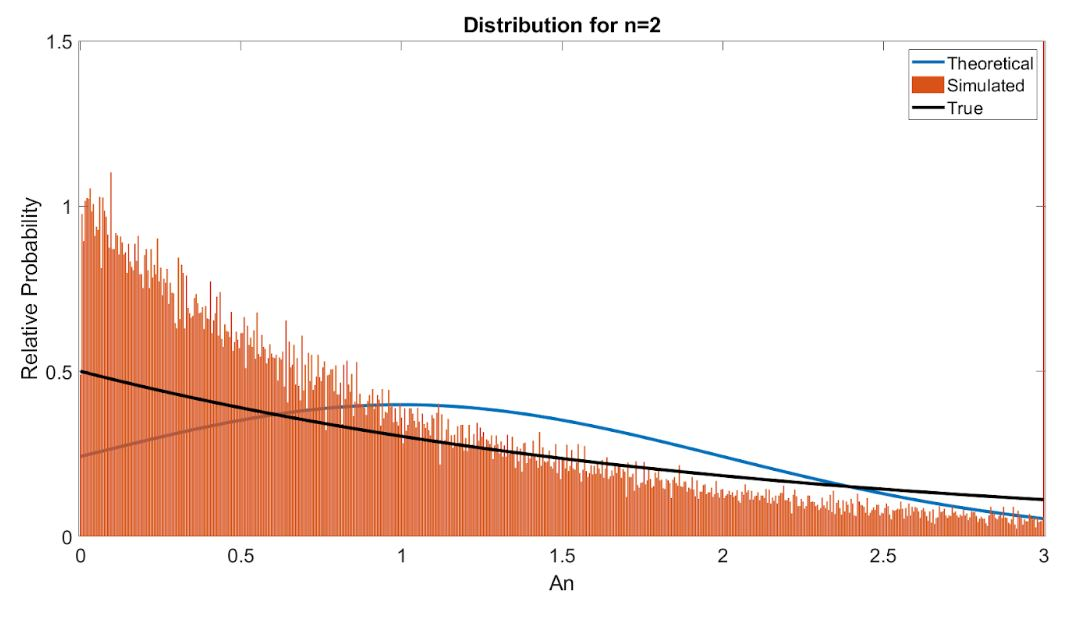
\includegraphics[scale=1.0]{Dpart1.jpg}
\caption{Comparing three PDFs using $n=2$}
\label{graph of $f(A_2)$}
\end{figure}
\newpage
\vspace*{1cm}
The distribution for both theoretical and simulated curves gets narrower as n increases. The main difference between the theoretical and simulated curves is the deviation. A higher deviation can be seen in the simulated PMF.
\begin{figure}[h!]
\centering
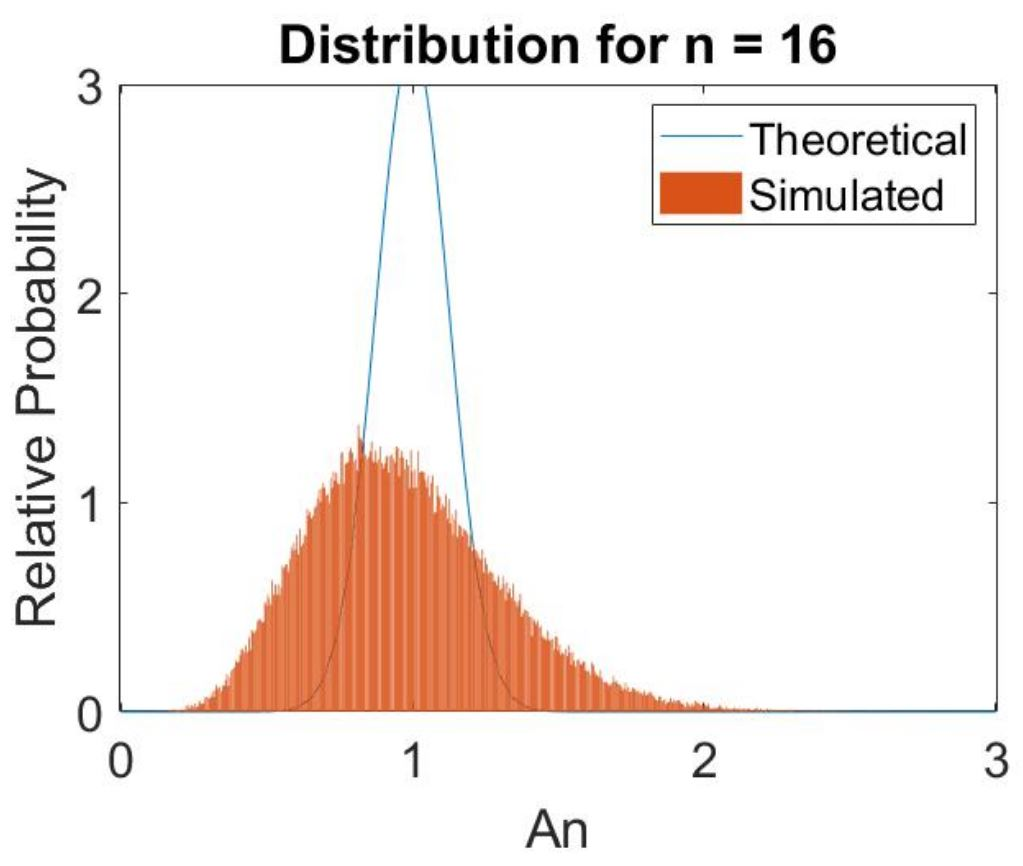
\includegraphics[scale=0.8]{Dpart1_2.jpg}
\caption{Simulated and Theoretical graph for $n = 16$}
\label{graph of $f(A_2)$}
\end{figure}

\vspace*{1cm}
\begin{figure}[h!]
\centering
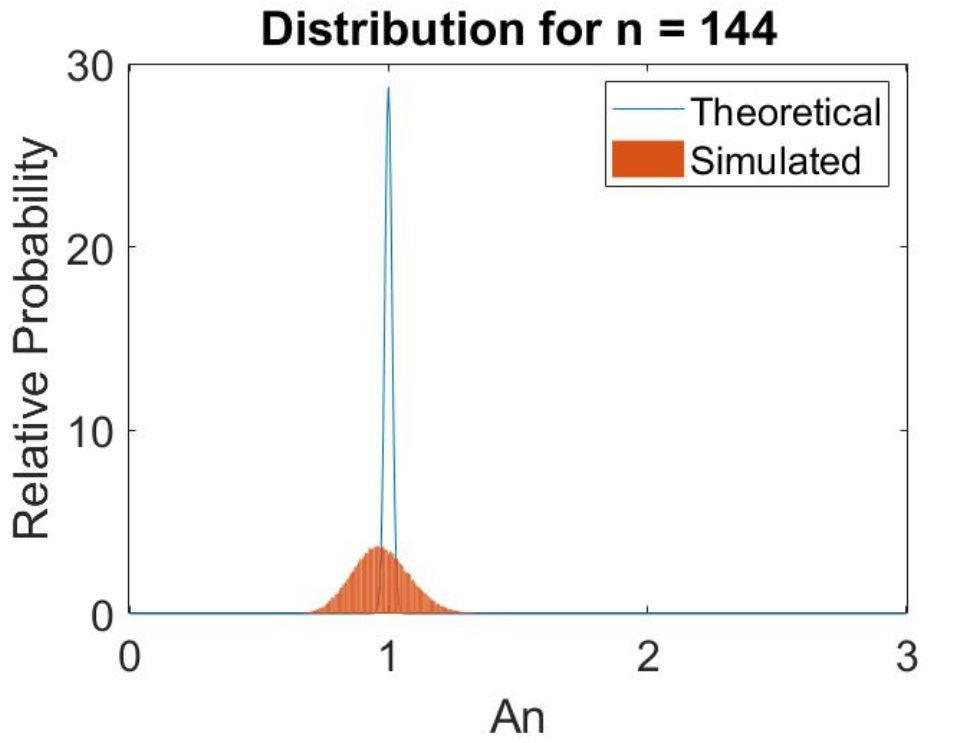
\includegraphics[scale=0.9]{Dpart1_3.jpg}
\caption{Simulated and Theoretical graph for $n = 144$}
\label{graph of $f(A_2)$}
\end{figure}

\newpage
\vspace*{1cm}
\section*{E) Approximate Theoretical PDF Using Geometric Mean}
To approximate the theoretical PDF, we set $G_n$ equivalent to the sigma product of $(x^2_i)^\frac{1}{n}$. Natural logging both sides, we then can transform the sigma product to a summation of $x^2$, and move the $(1/n)$ to the front. Substituting $\ln(G_n)$ as q, and $\ln(x^2)$ as b, we can simplify the equation and compute the definite infinite integral of $\int_{-\infty}^{\infty} G_nf_{G_n}(x_i)dx_i$.
\[
\mathlarger{G_n = (\prod_{i = 1}^{n}x^2_i)^\frac{1}{n}}
\]
\[
\mathlarger{\ln{G_n} = \frac{1}{n}\sum_{i = 1}^{n}(\ln{x^2_i})}
\]
\[
\mathlarger{\ln(G_n) = q, \ln{x^2} = b}
\]
\[
\mathlarger{q = \frac{1}{n}\sum_{i = 1}^{n}b_i = E(b)}
\]
\[
\mathlarger{E(G_n) = \int_{-\infty}^{\infty}G_nf_{G_n}(x_i)dx_i}
\]
\[
\mathlarger{[\int_{0}^{\infty}y^\frac{1}{n}\frac{1}{\sqrt{2\pi y}\sigma}e^\frac{-y}{2\sigma^2}dy]^n}
\]
\center Using substitutions to mimic the integral table $\mathlarger{x_1 = \frac{1}{n}-\frac{1}{2}}$, $\mathlarger{A = \frac{1}{2\sigma^2}}$, $\mathlarger{B=\frac{1}{\sqrt{2\pi}\sigma}}$
\[
\mathlarger{[B\int_{0}^{\infty}y^{x_1} y^\frac{-1}{2}e^{-Ay}dy]^n}
\]
\raggedright Simplifying further:
\[
\mathlarger{[B\int_{0}^{\infty}y^{x_1}e^{-Ay}dy]^n}
\]
We referred to the integral tables to find a similar integral to ours and found a Gamma result.
\begin{figure}[h!]
\centering
\includegraphics[scale=0.75 ]{PartE_2.jpg}
\end{figure}
\[
\mathlarger{\overline{G_n} = [\frac{\frac{1}{\sqrt{2\pi}\sigma}\Gamma{(\frac{1}{n}-\frac{1}{2}+1})}{(\frac{1}{2\sigma^2})^{\frac{1}{n}-\frac{1}{2}+1}}]^n}
\]
\[
\mathlarger{=[\frac{\frac{1}{\sqrt{2\pi}\sigma}\Gamma{(\frac{1}{n}+\frac{1}{2}})}{\frac{1}{(2\sigma^2)^{\frac{1}{n}+\frac{1}{2}}}}]^n}
\]
To remove Gamma from our equation we used the substitution $\Gamma(N) = (N - 1)!$ to get a simplified equation.
\[
[(2\sigma^2)^{1+\frac{n}{2}}((\frac{1}{n}-\frac{1}{2})!)(\frac{1}{\sqrt{2\pi}\sigma})]^n
\]
We used Desmos to carry out the calculations. As you can see from the table below, our means match up with our Figure 8.
\newpage
\vspace*{1cm}
\begin{figure}[h!]
\centering
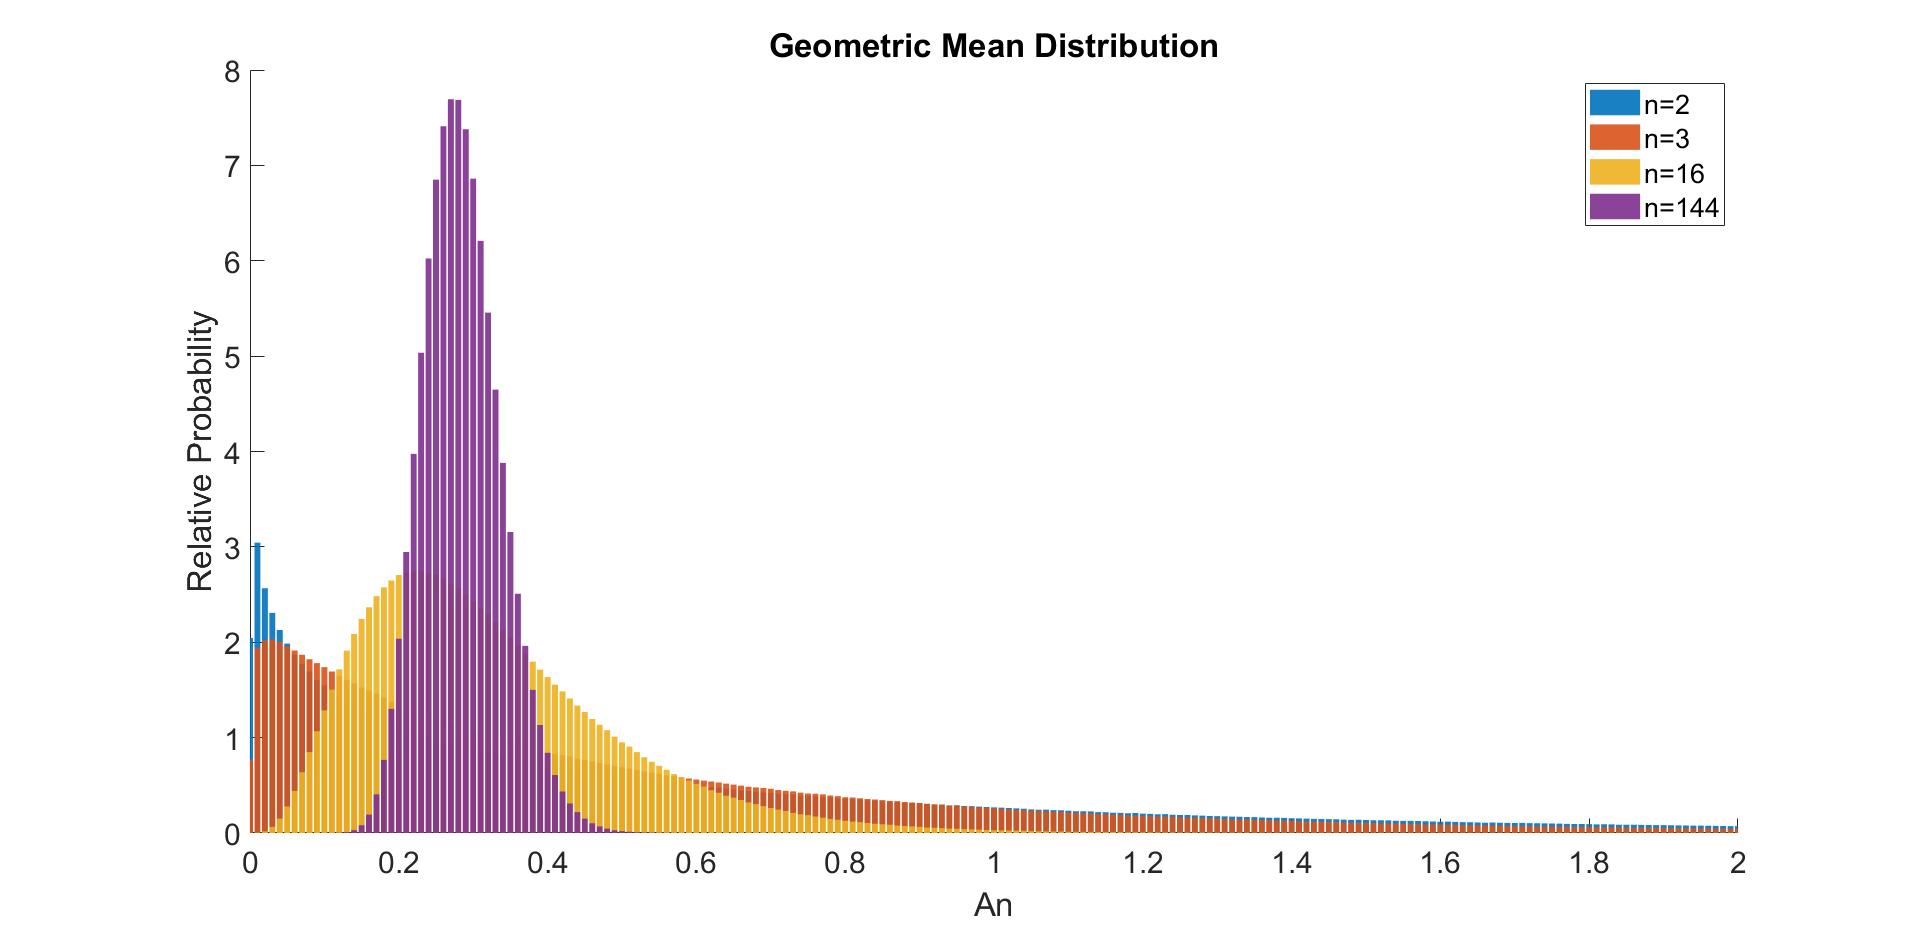
\includegraphics[scale=0.25]{PartE.jpg}
\caption{Simulated and Theoretical Graph for Geometric Mean}
\label{graph of $f(A_2)$}
\end{figure}
\begin{table}[!htpb]
\centering
\begin{tabular}{@{}lcccc@{}}
\toprule
\multicolumn{5}{c}{\textbf{Standard Deviation and Expectation for $G_n$}} \\ \midrule
\multicolumn{1}{c}{\textbf{\begin{tabular}[c]{@{}c@{}}\end{tabular}}} & \textbf{\begin{tabular}[c]{@{}c@{}}n = 2\end{tabular}} & \textbf{\begin{tabular}[c]{@{}c@{}}n = 3\end{tabular}} & \textbf{\begin{tabular}[c]{@{}c@{}}n = 16\end{tabular}} & \textbf{n = 144} \\ \midrule
Sim Standard Deviation & 0.7714 & 0.5538 & 0.1744 & 0.0527\\
Sim Expectation & 0.002 & 0.026 & 0.222 & 0.274\\
Theoretical Stand Dev & 0.637 & 0.517 & 0.324 & 0.286
\bottomrule
\end{tabular}
\end{table}

%%%%%%%%%%%%%%%%%%%%%%%%%%%%%%%%%%%%%%%%%%%%%%%%%%%%%%%%%
%%%%%%%%%%%%%% Appendix / MatLab Code %%%%%%%%%%%%%%%%%%%
%%%%%%%%%%%%%%%%%%%%%%%%%%%%%%%%%%%%%%%%%%%%%%%%%%%%%%%%%

\newpage
\vspace*{1cm}
\center\section*{Appendix}
				%%% Matlab part C using X^2. %%%
\vspace*{1cm}
\raggedright\subsection*{Matlab part C using $X^2$}
\begin{lstlisting}
%%% Matlab part C using X^2. %%%
clear all
sz = 0.01;
x=-3:sz:3;
y = [0:(.01/2):3];
n = 16;

% theoretical pdf of standard norm.
y1=normpdf(x, 0, 1);

% theoretical pdf of Y
fA = normpdf(y, 1, 2/n);
plot(y,fA,'LineWidth', 3);
hold on

%fy = 1./(sqrt(2*pi*y)).*exp(-y./2);

samp=100000;
for samples = 1:samp
    for index = 1:n
        
        y1 = y1/sum(y1); % Make sure probabilites add up to 1.
        cp = [0, cumsum(y1)];
        r = rand;
        ind = find(r>cp, 1, 'last');
        randx = x(ind);                   
        %https://www.mathworks.com/matlabcentral/answers/506654-select-random-
        %number-from-an-array-with-probabilities
        xsamp(index)=randx;
    end
    
    An(samples)=(1/n)*sum(xsamp.^2);
    
end
standardDev = std(An);
% simulated pdf of Y
[y3]=hist(An,y)/(samp*(sz/2));
bar(y,y3)

z=0:.01:3;
A2B = exp(-z/2)/2;
if n==2
plot(z,A2B,'K','LineWidth', 3)
end
title("Distribution for n=" + n)
ylabel('Relative Probability')
xlabel('An')
legend('Theoretical','Simulated','True')
set(gca,'FontSize',18)
%%%%%%%%%%%%%%%%%%%%%%%%%%%%%%%%%%%%%%%%%%
\end{lstlisting}


\newpage
\vspace*{1cm}
\raggedright\subsection*{Matlab part E using $X^2$}
\begin{lstlisting}
clear all
sz = 0.01;
x=-30:sz:30;
y = [0:sz:30];
n = [2 3 16 144];
binfac = 1;
yg = [-30:sz*binfac:30];
samp=1000000;

% theoretical pdf of standard norm.
y1=normpdf(x, 0, 1);

% theoretical pdf of Y
%fA = normpdf(y, 1, 2/n);
%plot(y,fA,'LineWidth', 3);
hold on
for i = 1:4
for samples = 1:samp
    ysamp=randn([1 n(i)]).^2;
    An(samples)=(prod(ysamp).^(1/n(i)));
    
end
standardDev = std(An);
% simulated pdf of An
[y3]=hist(An,yg)/(samp*(sz*binfac));
b1 = bar(yg,y3);
b1.FaceAlpha = 0.9;
end
z=0:.01:3;
A2B = exp(-z/2)/2;
if n==2
    plot(z,A2B,'K','LineWidth', 3)
end

%ylim([0, 1.5])
xlim([0, 2])
title("Geometric Mean Distribution")
ylabel('Relative Probability')
xlabel('An')
legend('n=2','n=3','n=16','n=144')
set(gca,'FontSize',18)
\end{lstlisting}





%%%%%%%%%%%%%%%%%%%%%%%%%%%%%%%%%%%%%%%%%%%%%%%%%%%%%%%%%
%%%%%%%%%%%%%% Responsibilities Table %%%%%%%%%%%%%%%%%%%
%%%%%%%%%%%%%%%%%%%%%%%%%%%%%%%%%%%%%%%%%%%%%%%%%%%%%%%%%
\begin{table}[!htpb]
\centering
\begin{tabular}{@{}cccc@{}}
\toprule
\multicolumn{4}{c}{\textbf{Responsibilities and Work}} \\ \midrule
\multicolumn{1}{c}{\textbf{\begin{tabular}[c]{@{}c@{}}Ethan Barnes\end{tabular}}} & \textbf{\begin{tabular}[c]{@{}c@{}}Deniz Misirlioglu\end{tabular}} & \textbf{\begin{tabular}[c]{@{}c@{}}Jared Rozell\end{tabular}} & \textbf{Riley Taylor} \\ \midrule
All Matlab & A and B & PDF matlab & Coding in LaTeX\\
PDF comparison & part E & . & Theoretical Part A\\
Part E & Gamma Explanation & . & Part E\\
\bottomrule
\end{tabular}
\end{table}
\vspace*{-0.5cm}
\center Note: Ethan, Deniz, and Riley all worked together on most parts
\end{document}